\chapter{Information-Theoretic Map Compression}
\label{chapter3}

The remaining chapters of this thesis introduce novel extensions to active perception
that make information-theoretic reward evaluation orders of magnitude more
efficient at the cost of information accuracy (Chapter~\ref{chapter4}), and allow the
robot to implicitly consider and avoid complex regions
in its local map while simultaneously planning informative paths (Chapter~\ref{chapter5}). Both
of these extensions originate from the observation that the information content
of a robot's sensor measurement depends on the environment
representation. In the case of OG maps, the cell resolution parameter shares an
intricate relationship with the robot's exploration behaviors.

One example of the relationship between OG cell resolution and exploration
behavior lies in the efficiency of raycasting. Most information-theoretic reward
functions (e.g. SMI and CSQMI) require simulating a beam-based sensor measurement from a future
position, which implicitly requires raycasting through the map. Intuitively, as
the resolution of cells in the map decreases, so too does the number of cells
that a raycast must traverse. Therefore the efficiency of information-theoretic reward evaluation
is a function of the cell resolution of the OG. For example, using the approximate
CSQMI technique from Charrow et al.~\cite{charrow2015icra}, this relationship is linear
(Fig.~\ref{fig:csqmi_timing}). As will be shown, the resolution of an OG map can typically be halved several
times before a significant amount of information about free and occupied space
is lost. However, sequentially halving the resolution exponentially increases the
speed of computing CSQMI, regardless of sensor range or number of beams. This
can be seen by holding range constant and tracing vertical lines down Fig.~\ref{fig:csqmi_timing}.

\begin{figure}
  \centering
  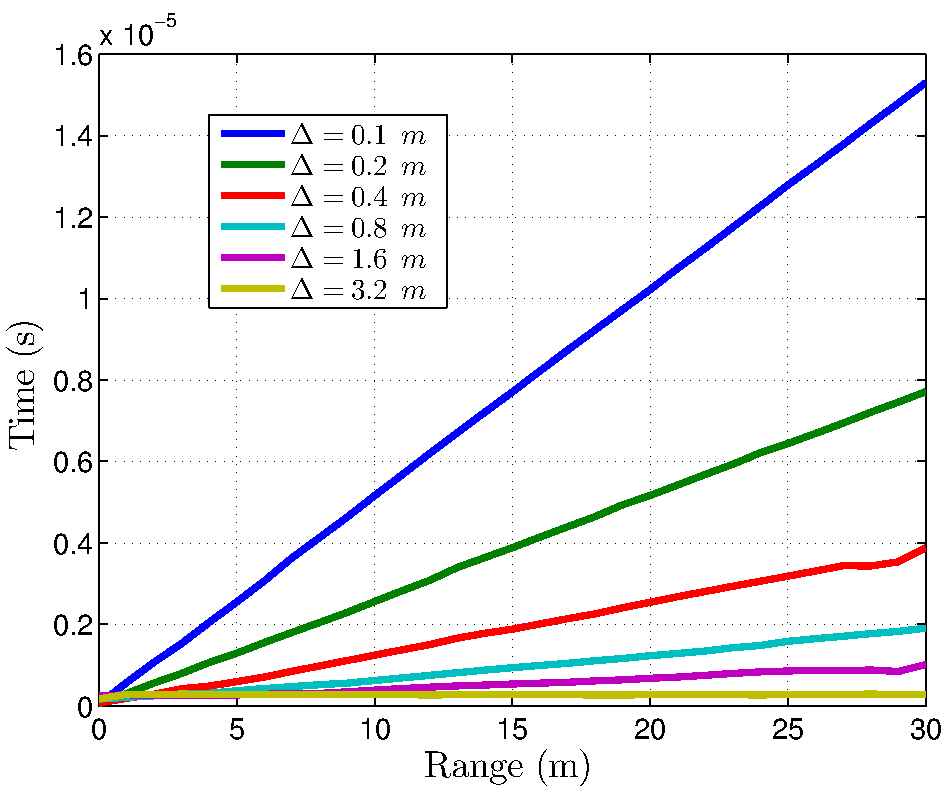
\includegraphics[width=0.65\textwidth]{csqmi_timing.pdf}
  \caption[Time complexity of computing CSQMI for a varying map resolution.]{Time (median of $10^5$ samples) to evaluate CSQMI for a
    single beam is linear in both the OG resolution $\Delta$, and
  the measurement range. \label{fig:csqmi_timing}}
\end{figure}

The incentive for increasing the efficiency of information-theoretic exploration
is clear and immediate; any reduction to the time required to evaluate an
information-theoretic reward function will enable robots to explore at higher
speeds, in turn allowing them to initialize (build a map) faster, or clear a
building for threats more quickly. However, at present, there is no clear choice
of algorithm for compressing an OG from one resolution to another.

Several others have proposed strategies for map compression. The OctoMap
framework~\cite{wurm2010octomap} builds an octree data structure to efficiently store the
expected occupancy of cells in an environment without allocating memory for a
large 3D grid. Jeong et al.~\cite{im2010real} compress an OG by representing it with
wavelets using the Haar wavelet transform. Kretzschmar et
al.~\cite{kretzschmar2012information} compress
pose graph maps by examining the SMI between the pose
graph and sensor measurements. Most related to the formulations in this chapter is the
work by Einhorn et al.~\cite{einhorn2011finding}, which adaptively chooses an OG resolution for
individual cells by determining which cells are intersected by measurements.

Instead of using a previous approach, the following chapter describes the first main contribution of this
thesis: a novel strategy for OG compression using the Principle of Relevant
Information~\cite{principe2010information}. In contrast to previous works on map
compression, this strategy approaches the compression problem from an information theory
perspective, optimizing a functional that describes the distortion between the
map and its compressed form. The proposed map compression strategy yields an
exceedingly simple compression algorithm that is founded on rate
distortion theory. This compression algorithm acts as a basis for the
active perception extensions introduced in Chapters~\ref{chapter4} and~\ref{chapter5}.

\section{The Principle of Relevant Information}

The OG compression problem can be formulated as an information-theoretic optimization
using the Principle of Relevant Information (PRI). PRI is a technique for learning a
reduced representation $\hat{X}$ of a random variable $X$ such that both the entropy of
$\hat{X}$ and the divergence of $\hat{X}$ with respect to the original data are minimized.
%
\eq{
    J(\hat{X})
    &=
    \min_{\hat{X}}
    (
    \text{H}_{\alpha}(\hat{X})
    +
    \lambda
    \text{D}_{\alpha}(X \vert \vert \hat{X})).
    \label{eq:pri_general}
}

The two terms of the PRI cost function are R\'{e}nyi's $\alpha$-entropy, which describes
the amount of uncertainty in its argument, and R\'{e}nyi's $\alpha$-divergence, which is a
distance measure describing distortion between $p(x)$ and $p(\hat{x})$. These terms simplify
to the more common Shannon entropy and Kullback-Leibler divergence for $\alpha = 1$. The
variational parameter $\lambda$ controls the amount of distortion in the compressed data.
Following Principe et al., we choose to minimize the $\text{H}_{2}$ entropy and
Cauchy-Schwarz divergence. For discrete random variables $X$ and $\hat{X}$,
%
\eq{
    \text{H}_{2}(\hat{X}) &= -\log \sum_{i} p^{2}(\hat{x}_{i}),
}
\eq{
    \text{D}_{\text{CS}}(X \vert \vert \hat{X}) =
    \log
    \frac{
    \sum_{i} p^{2}(x_{i}) \sum_{i} p^{2}(\hat{x_{i}})
    }
    {
    \left(\sum_{i} p(x_{i})p(\hat{x_{i}})\right)^{2}
    }.
    \label{eq:cs_divergence}
}

The cost function in~\eqref{eq:pri_general} is then:
%
\eq{
    (1-\lambda)\, \text{H}_{2}(\hat{X})-\lambda 2 \log \sum_{i}
    p(x_{i})p(\hat{x_{i}}) - \lambda \text{H}_{2}(X).
    \label{eq:cost_func}
}

The third term has no influence on the minimization over $\hat{X}$, and can be ignored. We
choose to give equal weight to the entropy and divergence, and optimize for $\lambda=1$.
Noting that logs and quadratic functions increase monotonically for positive arguments,
and noting that the summand in the second term of~\eqref{eq:cost_func} must be positive,
the optimization can be simplified to:
%
\eq{
    J(\hat{X})
    &=
    \max_{\hat{X}}
    \sum_{i} p(x_{i}) p(\hat{x}_{i}).
    \label{eq:pri_specific}
}

\begin{figure}
    \centering
    \begin{subfigure}[t]{0.45\textwidth}
        \centering
        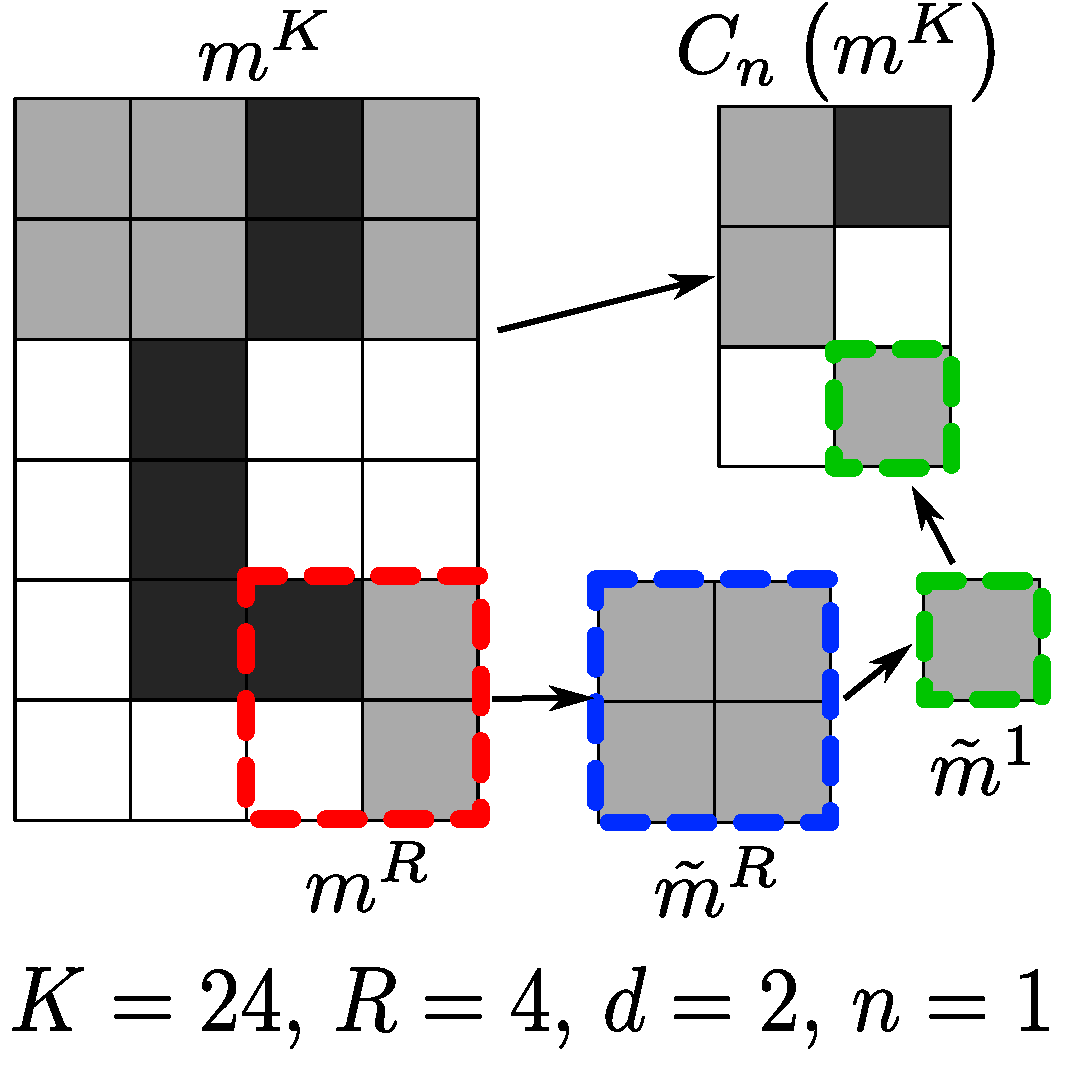
\includegraphics[height=5.3cm]{map_compression.pdf}
        \caption{OG compression sequence \label{fig:pri_compression1}}
    \end{subfigure}
    \hfill
    \begin{subfigure}[t]{0.45\textwidth}
        \centering
        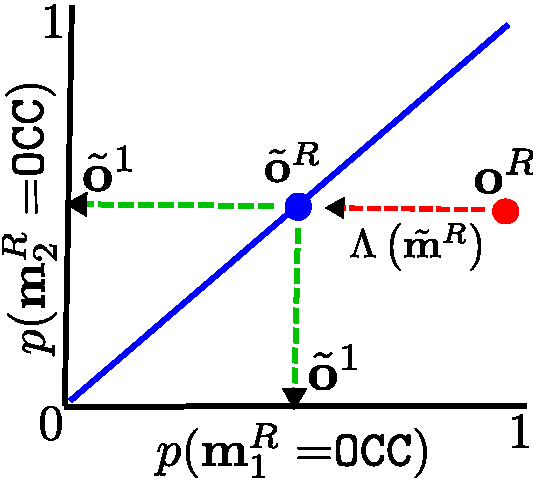
\includegraphics[height=5.3cm]{compression.pdf}
        \caption{Probability space of the top two grid cells
        in $m^{R}$ in~\ref{fig:pri_compression1} \label{fig:pri_compression2}}
    \end{subfigure}
    \caption[Occupancy grid compression sequence.]{For each square (cubic in 3D) region $m^{R}$ in the uncompressed OG $m^{K}$,
    the PRI optimization finds a random variable $\tilde{m}^{R}$ that
    minimizes~\eqref{eq:pri_general} and is constrained to have uniform occupancy
    probability $\tilde{o}^{R} = (\tilde{o}^{1}, \dots, \tilde{o}^{1})$.
  \label{fig:pri_compression}}
\end{figure}


\section{Framing Map Compression as an Optimization}

To apply the PRI optimization to OG compression, let $X$ be an OG $m^{K}$ with $K$ cells.
The problem must be constrained in three ways. First, because OGs encode a 2D or 3D geometry,
$\hat{X}$ must represent $X$ well in local regions. Compression over the map can therefore
be accomplished by performing compression in many small independent square (cubic in 3D)
regions $m^{R} \subseteq m^{K}$, assuming individual grid cell occupancies are independent.
Second, we consider only the set of compressions that reduce OG cell count in each dimension
by factors of two. Therefore an OG $m^{K}$ will be compressed to an OG $m^{2^{-dn}K}$, where
$d$ is the OG dimension and $n$ is the number of $2\times$ compressions in each dimension. The
set of compressions with this property can be expressed as:
%
\eq{
    C_{n}(m^{K}) \equiv m^{2^{-dn}K}, \quad n \in \mbb{N}_{0},
}

where superscripts denote cell count and where a compression of $n=0$ gives the original OG:
$C_{0}(m^{K}) = m^{K}$. Both $m^{K}$ and $C_{n}(m^{K})$ will have the same metric dimensions,
but will have different cell edge lengths and cell counts when $n \ge 1$. Finally, we enforce
that $\hat{X}$ must also be an OG. Since $\text{D}_{\text{CS}}(X\vert \vert \hat{X})$ may only
be computed for two random variables with the same support set, we use the PRI to find a random
variable $\tilde{m}^{R}$ that has uniform occupancy probabilities, and then reduce its dimension
to one, yielding a single grid cell $\tilde{m}^{1}$ (Fig.~\ref{fig:pri_compression}). Combining the
single-cell $\tilde{m}^{1}$ variables from independent regions yields the compressed OG $C_{n}(m^{K})$.

Rather than directly maximizing~\eqref{eq:pri_specific} over $\tilde{m}^{R}$, we are interested in
finding the distribution $p(\tilde{m}^{R})$ corresponding to the maximum. $p(\tilde{m}^{R})$ is a
Bernoulli distribution, and is completely determined by its single parameter
$\tilde{o}^{1} = p(\tilde{m}^{R} = \{\texttt{OCC},\dots,\texttt{OCC}\}) = 1 -
p(\tilde{m}^{R} = \{\texttt{EMP},\dots,\texttt{EMP}\})$. Substituting the described
variables into~\eqref{eq:pri_specific},
%
\eq{
    \tilde{o}^{1}_{*} &=
    \argmax_{\tilde{o}^{1}}
    \sum_{M^{R}}
    p\left(m^{R} = M^{R}\right)p\left(\tilde{m}^{R}=M^{R}\right).
    \label{eq:pri_specific2}
}

\section{Solving the Optimization}

\begin{sidewaystable*}[t]
  \caption[A contingency table for occupancy grid compression distributions.]{Contingency table for a compression from the OG region $m^{R}$ to $\tilde{m}^{R}$. \texttt{O} and \texttt{E} stand for \texttt{OCC} and \texttt{EMP}. \label{tab:contingency}}
    \centering
    \scalebox{0.9}
    {
    \renewcommand{\arraystretch}{3}
    \begin{tabular}{| c | c | c | c | c | c | c | c |}
        \cline{3-7}
        \multicolumn{2}{c|}{}
        & \multicolumn{1}{c}{}
        & \multicolumn{1}{c}{}
        & \multicolumn{1}{c}{$\tilde{m}^{R}$}
        & \multicolumn{1}{c}{}
        & \multicolumn{1}{c|}{}
        & \multicolumn{1}{c}{}
        \\ \cline{3-8}
        \multicolumn{2}{c|}{}
        & \scalebox{0.9}{\texttt{E}, \texttt{E}, $\dots$, \texttt{E}} & \scalebox{0.9}{\texttt{E}, \texttt{E}, $\dots$, \texttt{O}} & $\dots$ & \scalebox{0.9}{\texttt{O}, \texttt{O}, $\dots$, \texttt{E}} & \scalebox{0.9}{\texttt{O}, \texttt{O}, $\dots$, \texttt{O}} & Total \\ \cline{1-4}\cline{6-8}
        \multirow{5}{*}{$m^{R}$}
        & \scalebox{0.9}{\texttt{E}, \texttt{E}, $\dots$, \texttt{E}} & $w_{2}\cdot(1-\tilde{o}^{1}) \cdot \prod_{i=1}^{R}(1-o_{i}^{R})$ & $0$ & $\dots$ & $0$ & $w_{3}\cdot \tilde{o}^{1}\cdot \prod_{i=1}^{R}(1-o_{i}^{R})$ & $\prod_{i=1}^{R}(1-o_{i}^{R})$\\ \cline{2-4}\cline{6-8}
        & \scalebox{0.9}{\texttt{E}, \texttt{E}, $\dots$, \texttt{O}} & $w_{1}\cdot(1-\tilde{o}^{1})\cdot o_{1}^{R}\cdot \prod_{i=2}^{R}(1-o_{i}^{R})$ & $0$ & $\dots$ & $0$ & $w_{4}\cdot\tilde{o}^{1}\cdot o_{1}\cdot \prod_{i=2}^{R}(1-o_{i}^{R})$ & $o_{1}\cdot \prod_{i=2}^{R}(1-o_{i}^{R})$\\ \cline{2-4}\cline{6-8}
        &
        \multicolumn{1}{c}{$\vdots$}
        &
        \multicolumn{1}{c}{$\vdots$}
        &
        \multicolumn{1}{c}{$\vdots$}
        &
        \multicolumn{1}{c}{$\ddots$}
        &
        \multicolumn{1}{c}{$\vdots$}
        &
        \multicolumn{1}{c}{$\vdots$}
        &
        \multicolumn{1}{c|}{$\vdots$} \\ \cline{2-4}\cline{6-8}
        & \scalebox{0.9}{\texttt{O}, \texttt{O}, $\dots$, \texttt{E}} & $ w_{1} \cdot (1-\tilde{o}^{1})\cdot (1-o_{1}^{R}) \cdot \prod_{i=2}^{R} o_{i}^{R}$ & $0$ & $\dots$ & $0$ & $w_{4}\cdot \tilde{o}^{1}\cdot (1-o_{1}^{R}) \cdot \prod_{i=2}^{R} o_{i}^{R}$ & $(1-o_{1}^{R}) \cdot \prod_{i=2}^{R} o_{i}^{R}$\\ \cline{2-4}\cline{6-8}
        & \scalebox{0.9}{\texttt{O}, \texttt{O}, $\dots$, \texttt{O}} & $w_{1}\cdot(1-\tilde{o}^{1})\cdot \prod_{i=1}^{R}o_{i}^{R}$ & $0$ & $\dots$ & $0$ & $w_{4}\cdot\tilde{o}^{1}\cdot \prod_{i=1}^{R}o_{i}^{R}$ & $\prod_{i=1}^{R}o_{i}^{R}$ \\ \cline{1-4}\cline{6-8}
        \multicolumn{1}{c|}{}
        & Total & $1-\tilde{o}^{1}$ & $0$ & $\dots$ & $0$ & $\tilde{o}^{1}$ & 1 \\ \cline{2-8}
    \end{tabular}
    }
\end{sidewaystable*}

Table~\ref{tab:contingency} shows a contingency table for a compression from the OG region $m^{R}$ to $\tilde{m}^{R}$. The middle columns of the contingency table have zero probability, since the $\tilde{m}^{R}$ must have a uniform cell probability to be able to reduce it to $\tilde{m}^{1}$ (i.e. $\tilde{o}^{R}_{i} = \tilde{o}^{R}_{j}=\tilde{o}^{1}\, \forall i,j \in 1,\dots,R$). In this section we are only interested in the marginal distributions (bottom-most row and right-most column), which are needed to determine~\eqref{eq:pri_specific2}. Substituting these,
%
\eq{
    \tilde{o}_{*}^{1}
    =
    &=
    \argmax_{\tilde{o}^{1}}
    \left(
    (1-\tilde{o}^{1}) \prod_{i=1}^{R}(1-o_{i}^{R})
    +\tilde{o}^{1} \prod_{i=1}^{R}o_{i}^{R}
    \right),
}

which is satisfied for
%
\eq{
    \tilde{o}_{*}^{1}
    &=
    \begin{cases}
    0           &\text{if} \ \prod_{i=1}^{R}\frac{o_{i}^{R}}{1-o_{i}^{R}} < 1 \\
    1           &\text{if} \ \prod_{i=1}^{R}\frac{o_{i}^{R}}{1-o_{i}^{R}} > 1 \\
    \frac{1}{2} &\text{otherwise}
    \end{cases},
    \label{eq:compression_cases}
}

where the last case applies in the limit as $\lambda \rightarrow 1^{+}$.

The PRI solution gives us a simple compression rule: if the product of cell occupancy likelihoods in a given region is greater than $1$, set the occupancy of the cell corresponding to that region in the compressed OG to $1$. Likewise set the value to $0$ if the product of likelihoods is less than $1$, and to $0.5$ if the product of likelihoods is $1$. Pragmatically, it is more reasonable to use the map's occupancy and free thresholds rather than $1.0$ and $0.0$. This variation corresponds to optimizing for $\lambda$ slightly greater than one, favoring minimal distortion to minimal entropy. Additionally, one may introduce a heuristic to increase the fraction of occupied cells that are preserved through compression by multiplying the right-hand sides of the inequalities in~\eqref{eq:compression_cases} by $\eta \in (0, 1)$. As $\eta$ decreases, occupied cells will be preserved through compression with higher frequency. For any application involving raycasting, it is especially important to include this heuristic, as vanishing occupied cells lead to poor ray termination.

Denoting $\pi^{R} \equiv \prod_{i=1}^{R}\frac{o_{i}^{R}}{1-o_{i}^{R}}$ and applying these modifications gives the $\sqrt{R}\times\sqrt{R}\rightarrow 1\times1$ (or $\sqrt[3]{R}\times\sqrt[3]{R}\times\sqrt[3]{R}\rightarrow 1\times1\times1$ in 3D) compression rule for each region $m^{R}$:
%
\eq{
    \tilde{o}_{*}^{1}
    &=
    \begin{cases}
    \frac{1}{2}             &\text{if} \ \pi^{R} = \eta \vee \pi^{R} = 1 \\
    p_{\text{free}}         &\text{if} \ \pi^{R} < \eta \wedge \pi^{R} \ne 1 \\
    p_{\text{occ}}          &\text{if} \ \pi^{R} > \eta \wedge \pi^{R} \ne 1
    \end{cases},
    \label{eq:compression_cases2}
}

where $p_{\text{occ}}$ and $p_{\text{free}}$ are the thresholds for occupied and free space in the OG implementation, respectively.

\section{Occupancy Grid Pyramids}

\section{Results}

\begin{figure}
  \centering
  \begin{subfigure}[t]{0.3\textwidth}
    \centering
    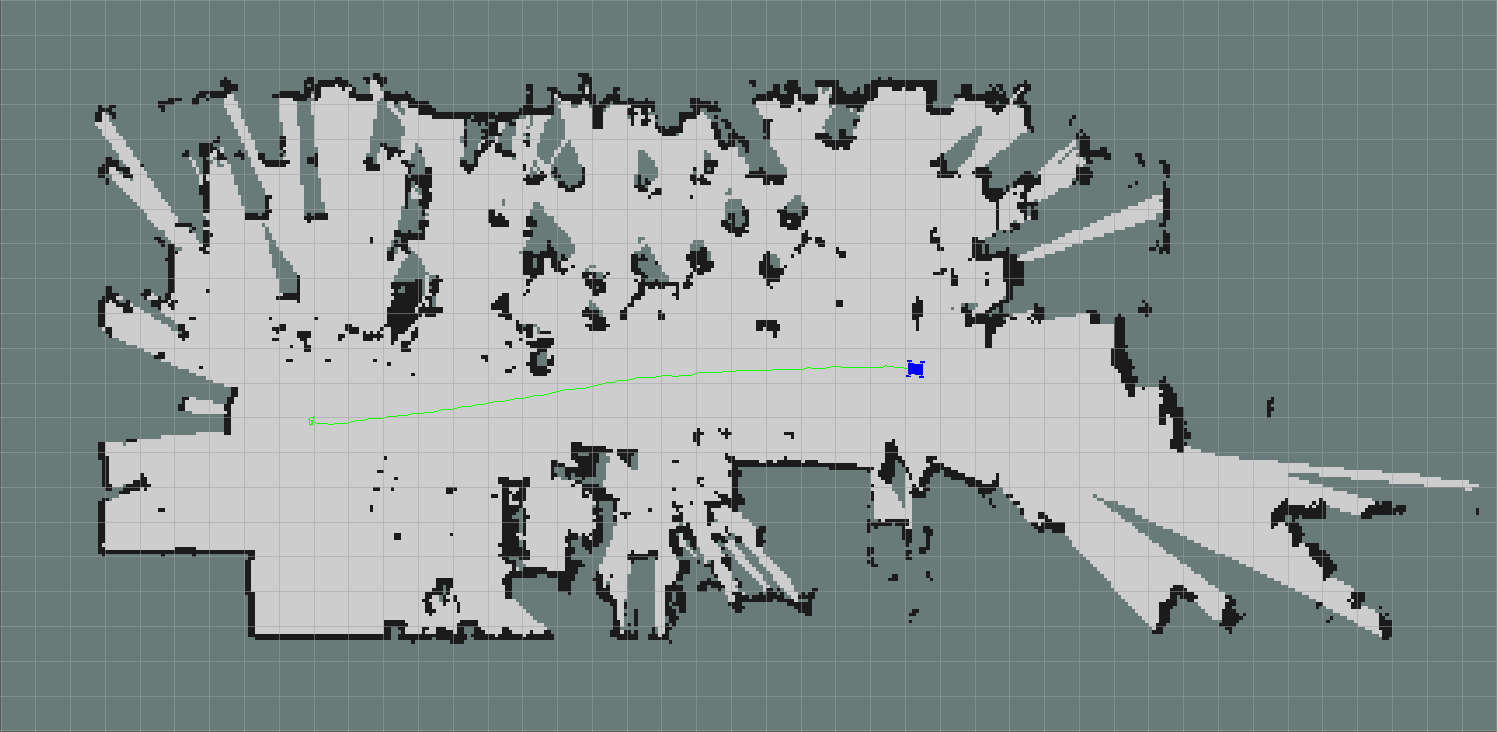
\includegraphics[angle=90, width=\textwidth]{compression0.png}
    \caption{\label{fig:}}
  \end{subfigure}
  \hfill
  \begin{subfigure}[t]{0.3\textwidth}
    \centering
    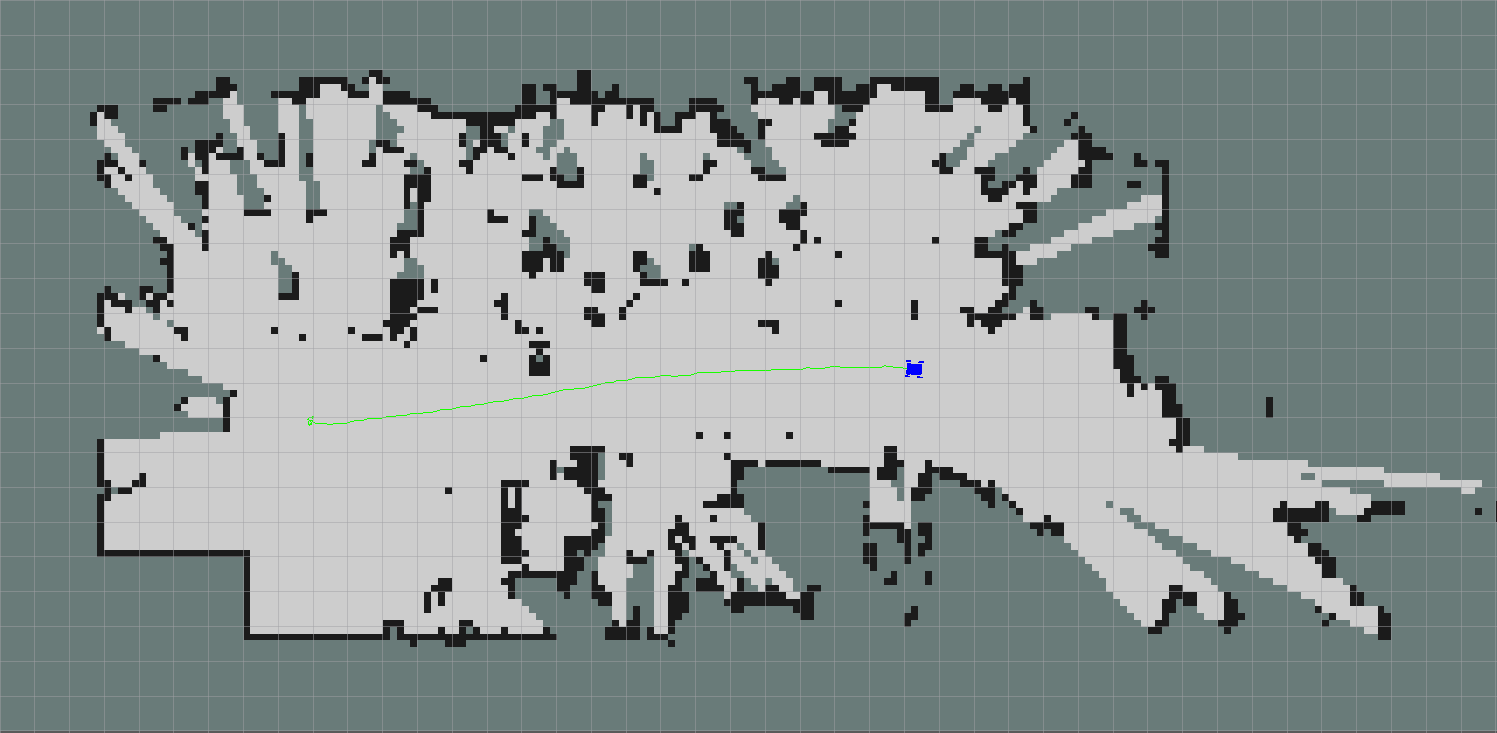
\includegraphics[angle=90, width=\textwidth]{compression1.png}
    \caption{\label{fig:}}
  \end{subfigure}
  \hfill
  \begin{subfigure}[t]{0.3\textwidth}
    \centering
    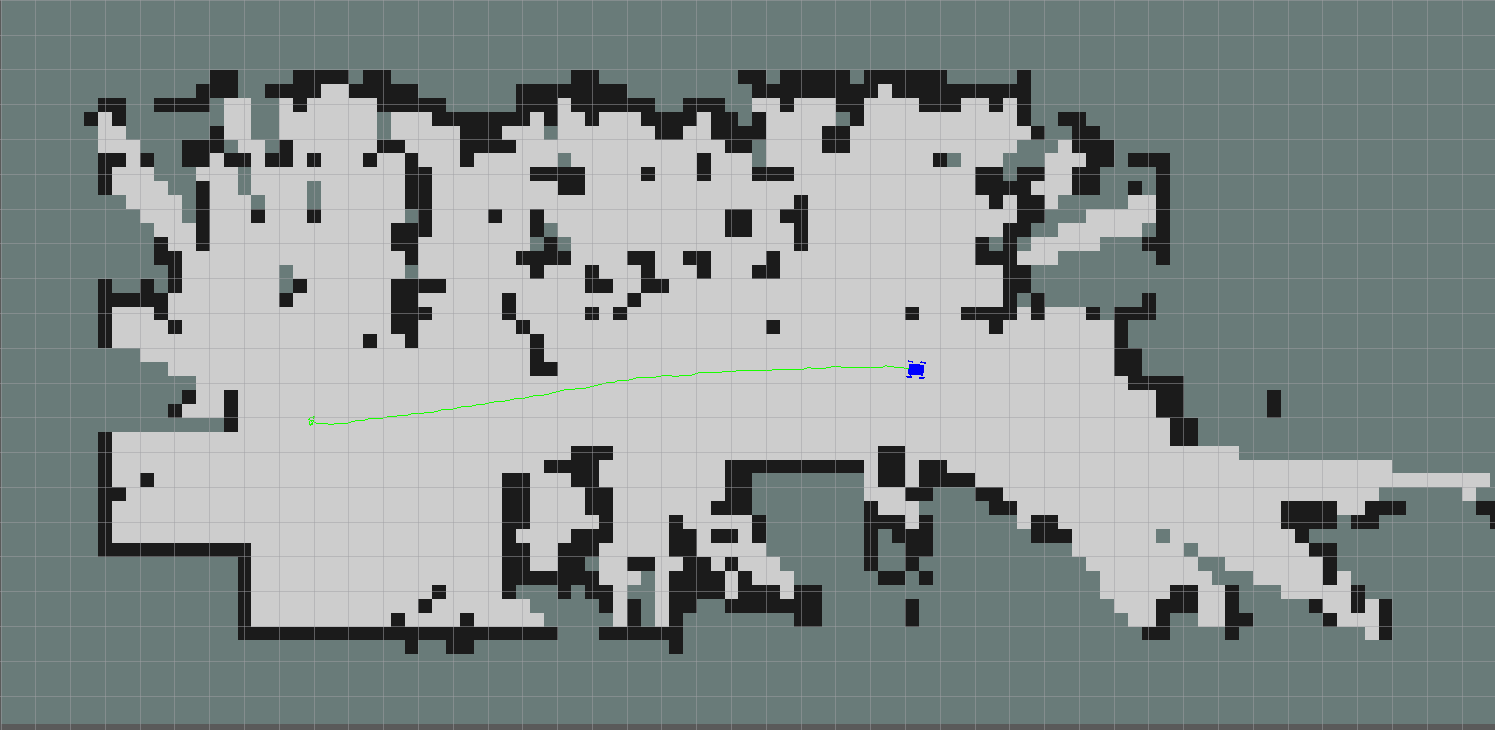
\includegraphics[angle=90, width=\textwidth]{compression2.png}
    \caption{\label{fig:}}
  \end{subfigure}
  \\
  \begin{subfigure}[t]{0.3\textwidth}
    \centering
    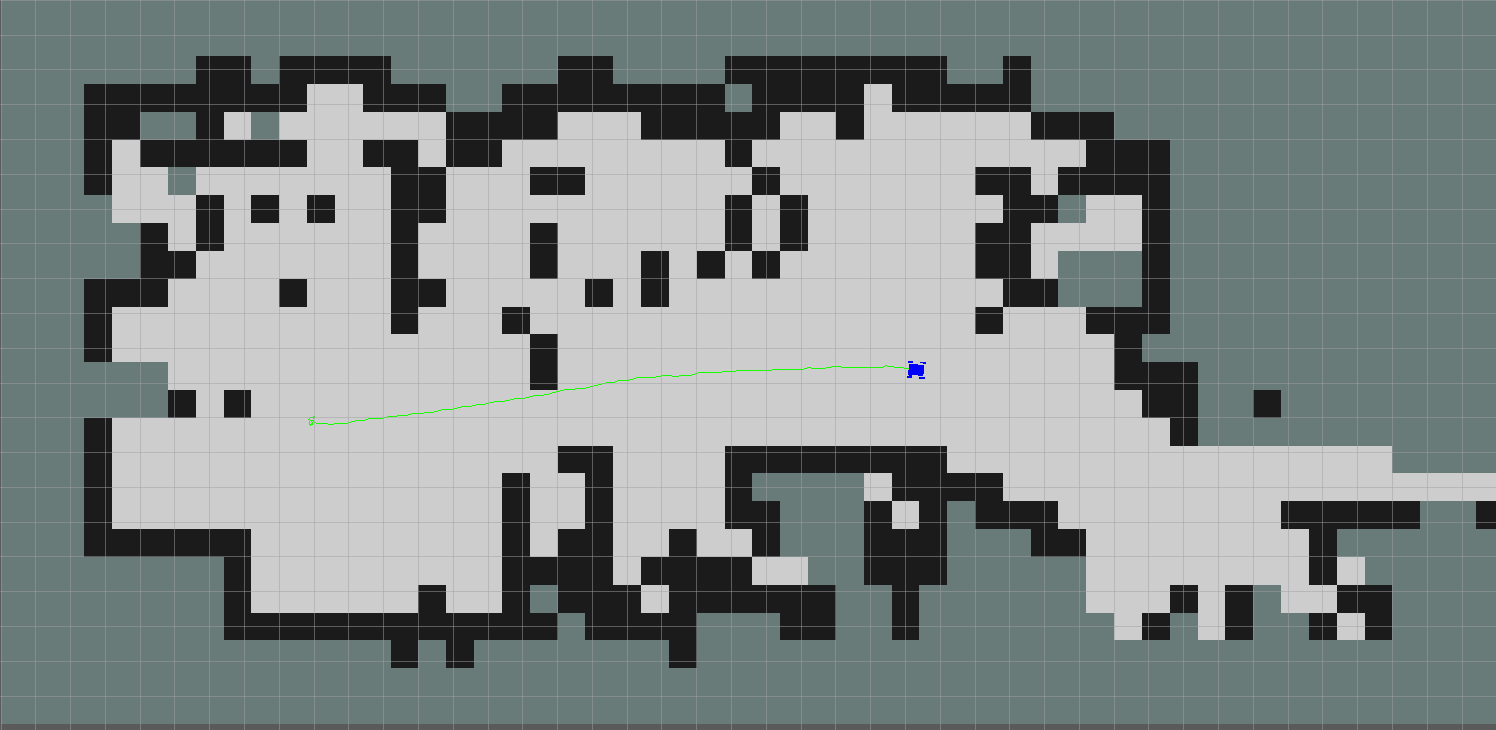
\includegraphics[angle=90, width=\textwidth]{compression3.png}
    \caption{\label{fig:}}
  \end{subfigure}
  \hfill
  \begin{subfigure}[t]{0.3\textwidth}
    \centering
    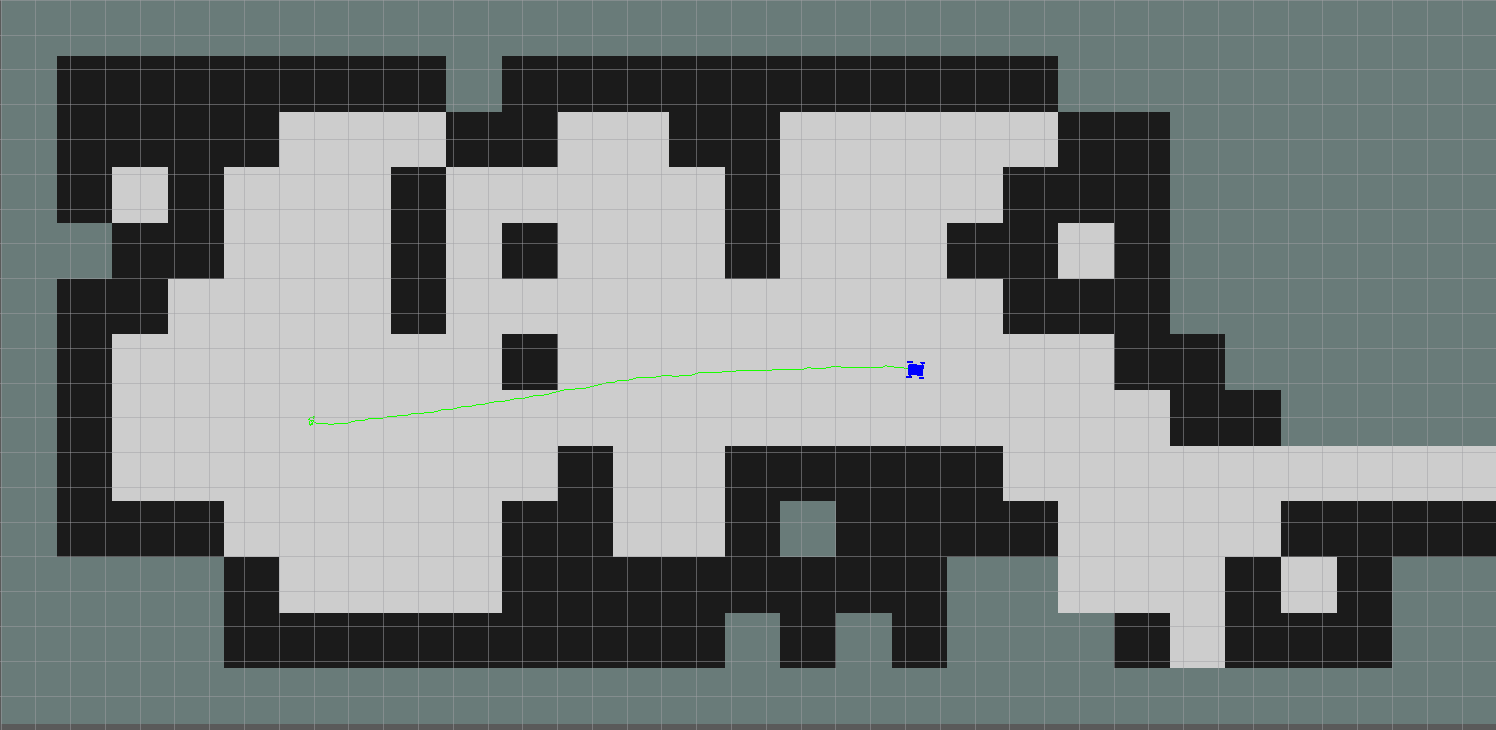
\includegraphics[angle=90, width=\textwidth]{compression4.png}
    \caption{\label{fig:}}
  \end{subfigure}
  \hfill
  \begin{subfigure}[t]{0.3\textwidth}
    \centering
    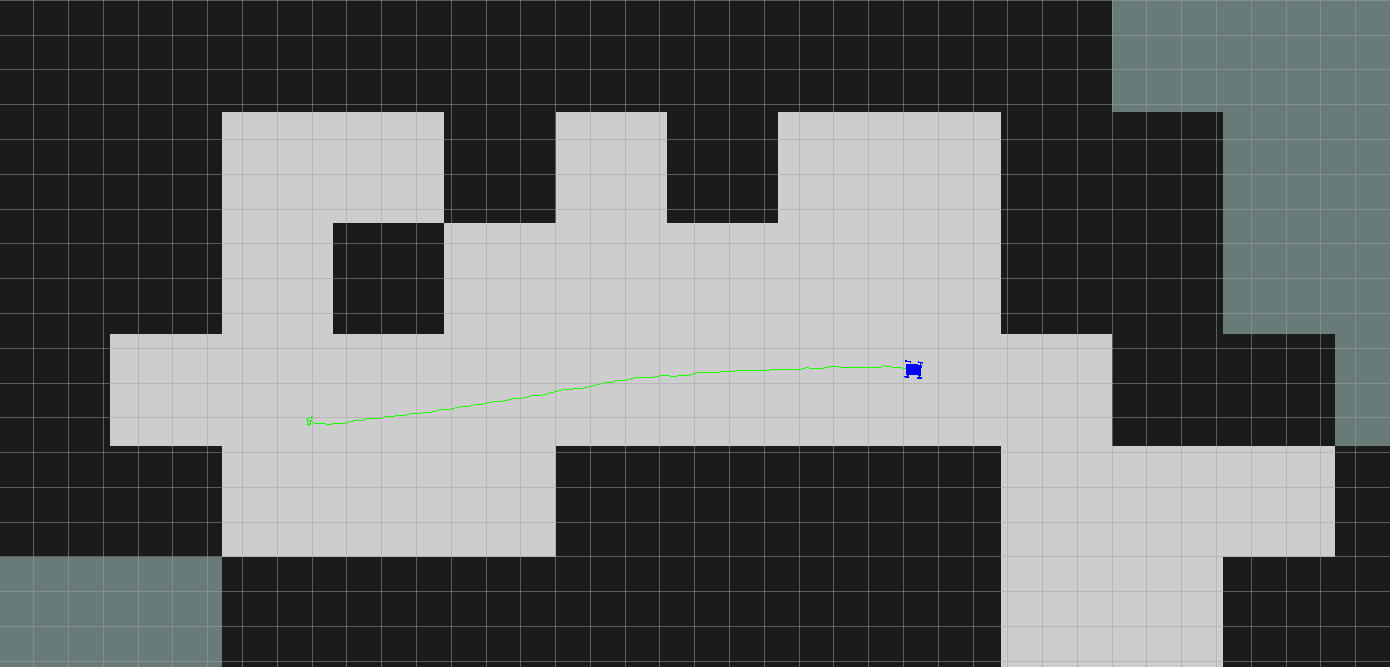
\includegraphics[angle=90, width=\textwidth]{compression5.png}
    \caption{\label{fig:}}
  \end{subfigure}
  \caption{\label{fig:}}
\end{figure}

\begin{figure}
  \centering
  \begin{subfigure}[t]{0.48\textwidth}
    \centering
    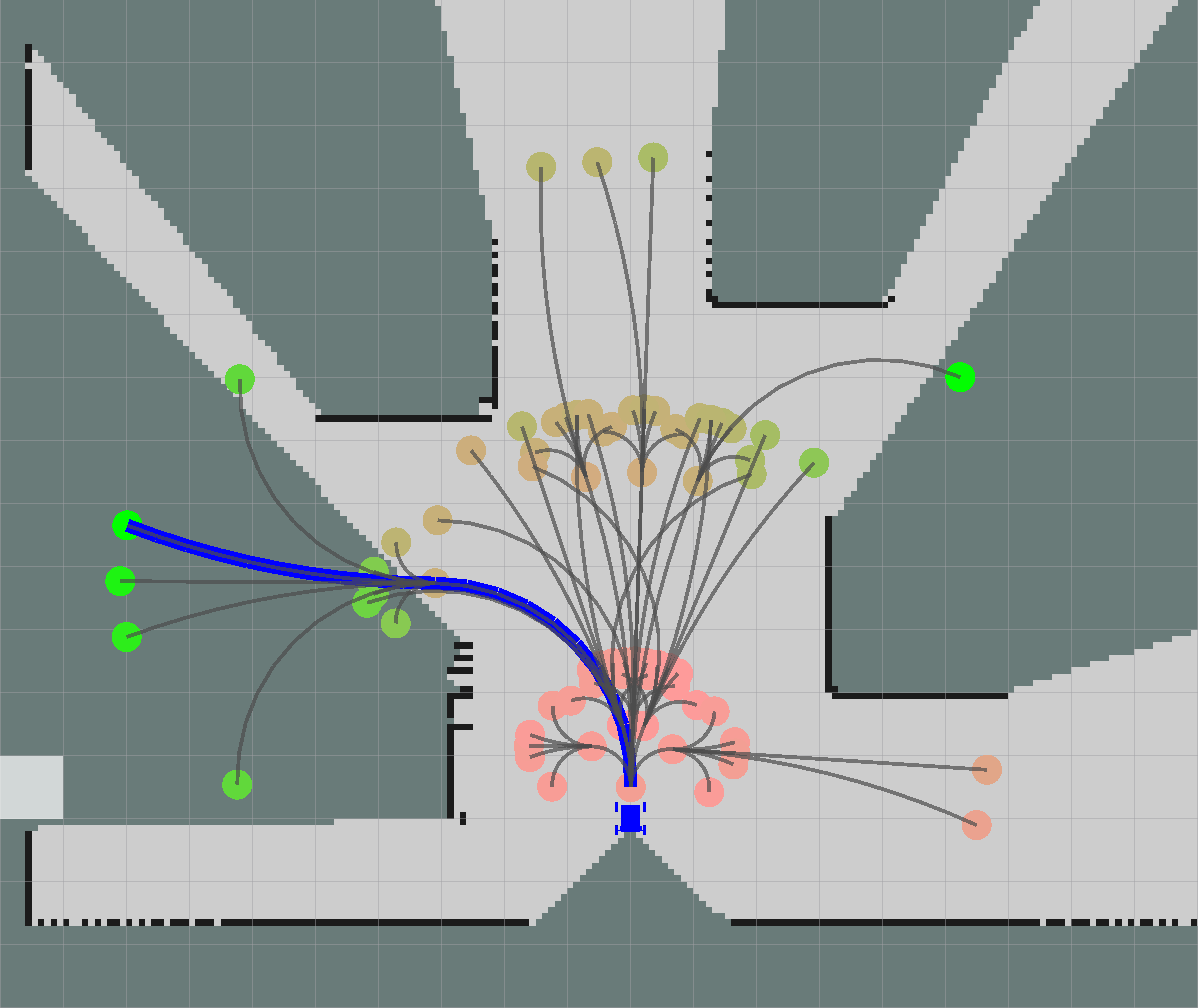
\includegraphics[width=\textwidth]{level0.png}
    \caption{\label{fig:}}
  \end{subfigure}
  \hfill
  \begin{subfigure}[t]{0.48\textwidth}
    \centering
    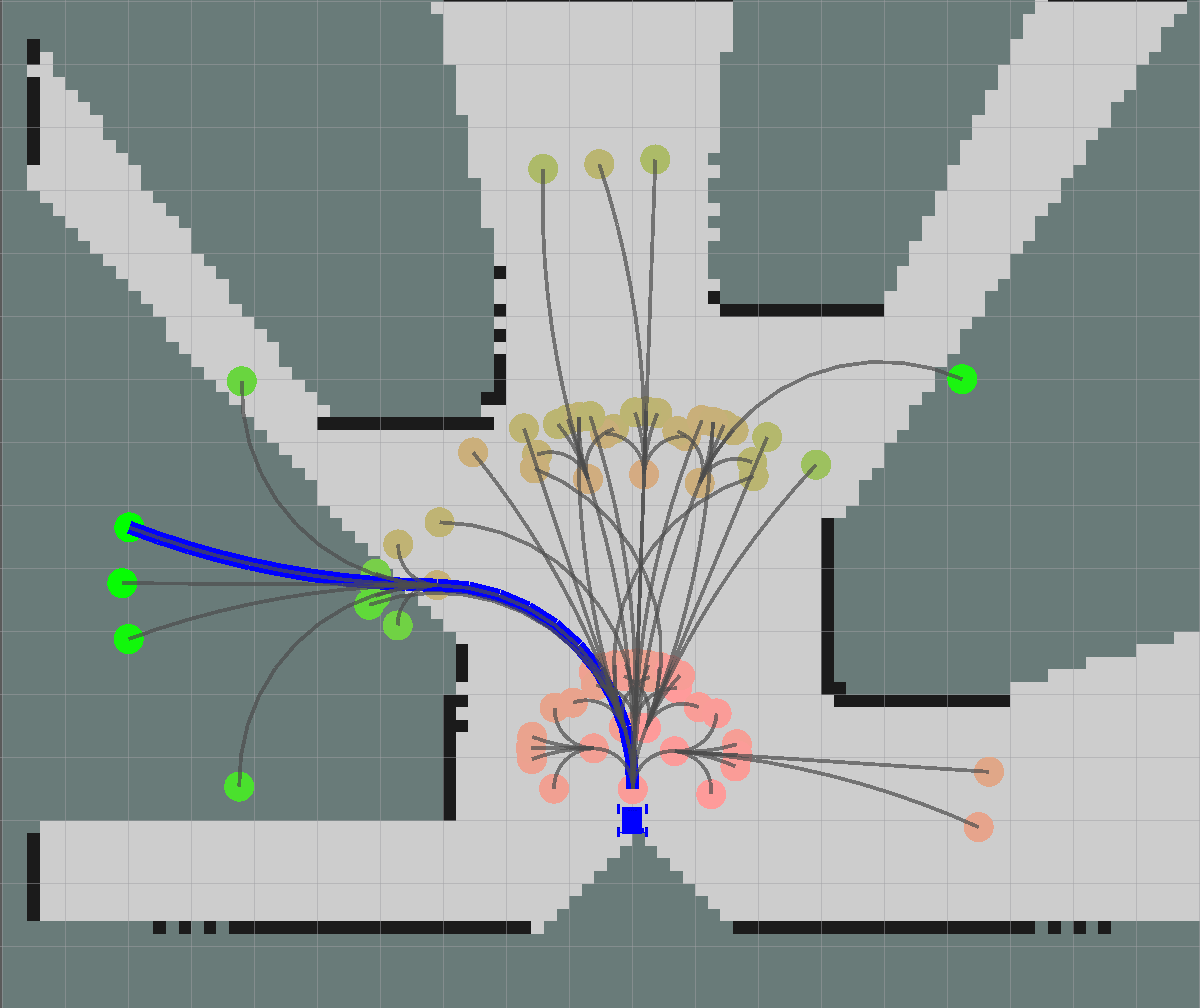
\includegraphics[width=\textwidth]{level1.png}
    \caption{\label{fig:}}
  \end{subfigure}
  \\
  \begin{subfigure}[t]{0.48\textwidth}
    \centering
    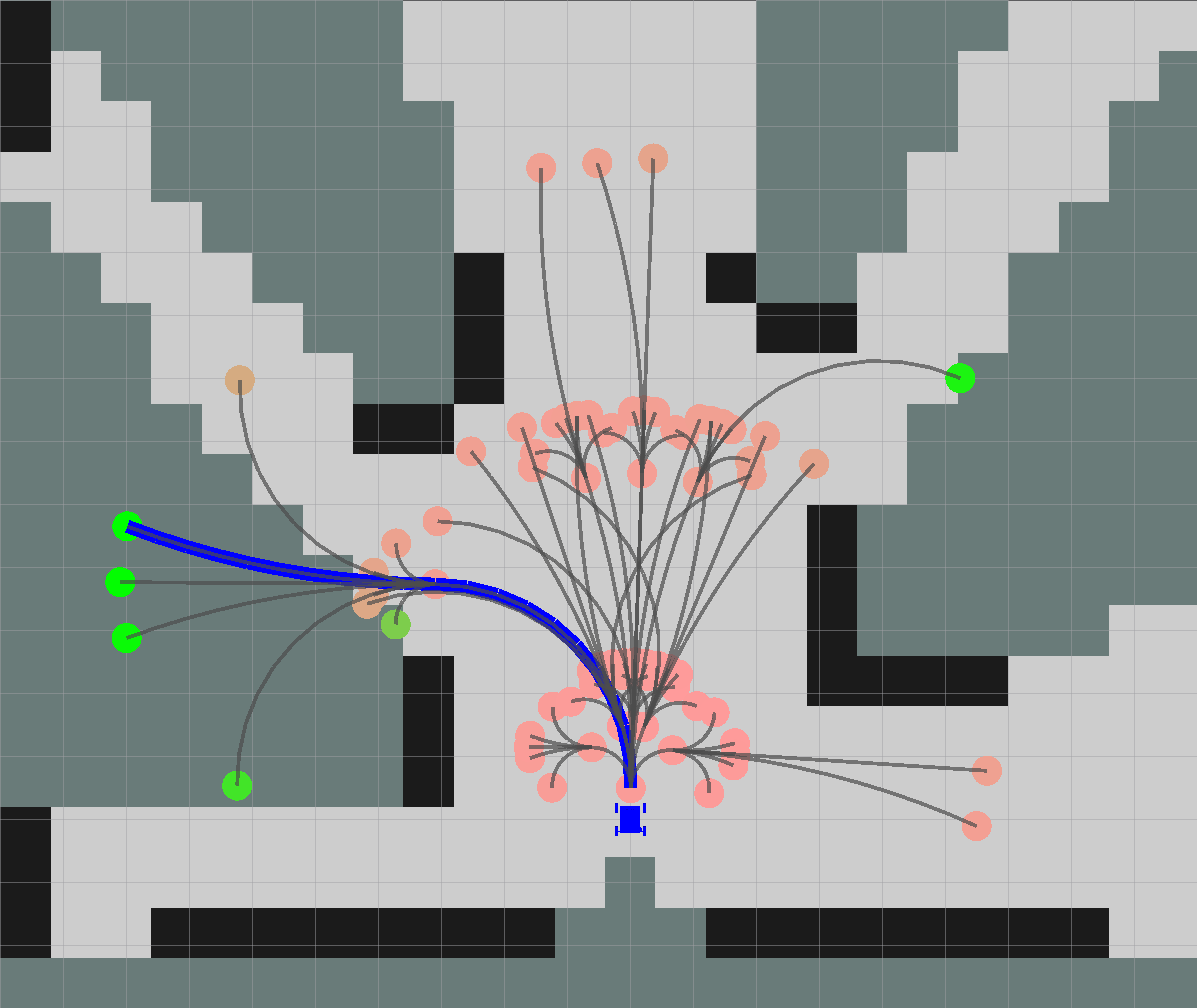
\includegraphics[width=\textwidth]{level3.png}
    \caption{\label{fig:}}
  \end{subfigure}
  \begin{subfigure}[t]{0.48\textwidth}
    \centering
    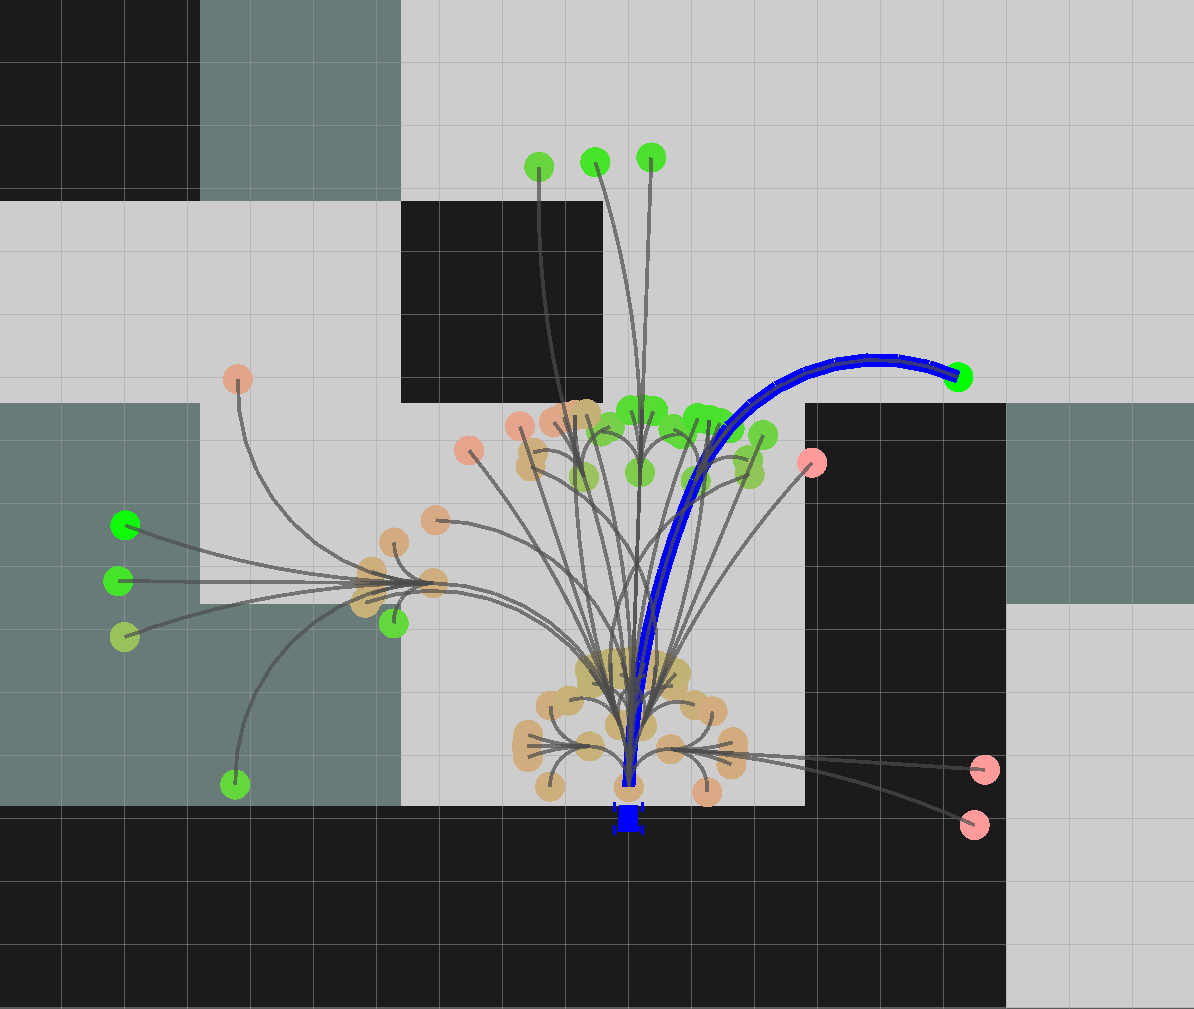
\includegraphics[width=\textwidth]{level5.png}
    \caption{\label{fig:}}
  \end{subfigure}
  \caption{\label{fig:}}
\end{figure}


\section{Chapter Summary}
